%% --------------------------------------------------------------
%%
%% K I L O N O V A
%%
%% --------------------------------------------------------------
\begin{frame}{Introduction}
\begin{tikzpicture}[overlay,remember picture]
\uncover<1->{ % <-> |
    \node (t1) [anchor=center,scale=1,opacity=1] at ([shift={(-3.6cm,1.3cm)}]current page.center){
        \parbox{0.60\textwidth}{
            Kilonova -- thermal EM counterpart to mergers, \\
            powered by the decay of produced elements
            \begin{itemize}
                \item Fast rise and decay
                \item Strong dependency on composition
                \item Dependency on the obs. angle
            \end{itemize}
    }};
}

\uncover<1->{ % <-> |
    \node (t1) [anchor=center,scale=1,opacity=1] at ([shift={(-3.6cm,-1.5cm)}]current page.center){
        \parbox{0.60\textwidth}{
            \AT{}, EM counterpart to \GW{}
            \begin{itemize}
            \item Extensive follow-up
            \item Early peak in blue bands (low $\kappa$)
            \item Late peak in red, IR, bands (high $\kappa$)
            \end{itemize}
    }};
}

\uncover<1->{ % <-> |
    \node (t1) [anchor=center,scale=1,opacity=1] at ([shift={(-3.6cm,-3.5cm)}]current page.center){
        \parbox{0.60\textwidth}{
            Several open questions
            \begin{itemize}
                \item Insufficient ejecta to explain early blue part.
            \end{itemize}
    }};
}

\uncover<1->{ % <-> |
    \node (img1) [anchor=center,scale=1,opacity=1] at ([shift={(4.0cm,-0.2cm)}]current page.center){
        \parbox{0.5\textwidth}{
            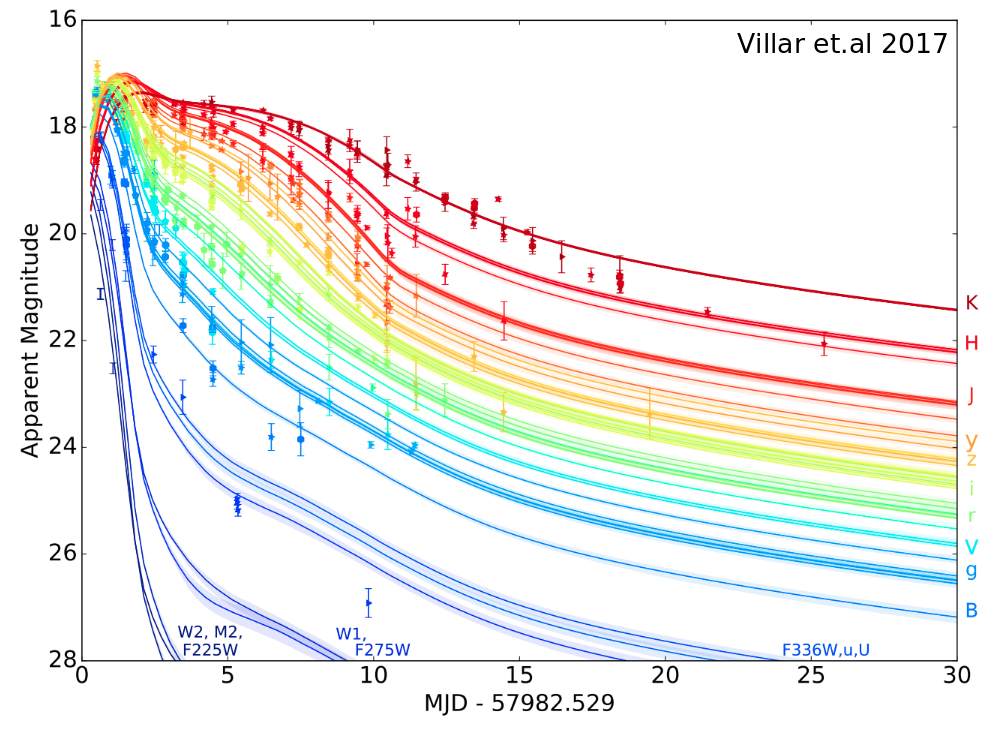
\includegraphics[height=5.5cm]{phd_figs/viller_mkn_model.png}
            
            
    }};
}
\end{tikzpicture}
\end{frame}

%\begin{frame}{Introduction} %% ---------- title 
%Thermal counterpart, powered by the decay of newly synthesized heavy elements %\citep[\eg][]{Li:1998bw,Kulkarni:2005jw,Metzger:2010,Roberts:2011,Metzger:2016pju,Wollaeger:2017ahm}
%The only unambiguous detection \AT{}
%%\citep{Arcavi:2017xiz,Coulter:2017wya,Drout:2017ijr,Evans:2017mmy,Hallinan:2017woc,Kasliwal:2017ngb,
%%    Nicholl:2017ahq,Smartt:2017fuw,Soares-santos:2017lru,Tanvir:2017pws,
%%    Troja:2017nqp,Mooley:2018dlz,Ruan:2017bha,Lyman:2018qjg}. 
%very well sampled.
%Distinguished blue/red components attributed to low/high opacity material, %\citep[\eg][]{Villar:2017wcc}
%%lanthanides $(58\leq Z \leq71)$ and actinides $(90\leq Z \leq 103)$, that have an open $f$-shell 
%or high/low $Y_e$ material
%%
%%Other candidates 
%%GRB130603B, \citep{Berger:2013wna,Tanvir:2013pia}, 
%%GRB060614 \citep{Jin:2015txa,Yang:2015pha}, 
%%GRB050709 \citep{Jin:2016pnm}. 
%
%%The peak luminosity \textit{Arnett's Law} \citep{Arnett:1982}.
%%In this simplified picture, three ingredients are required to understand the observations of \ac{kN}. 
%%These are 
%%\begin{itemize}
%%    \item The ejecta properties: $M$, $\upsilon$, $Y_e$,
%%    \item The composition of the expanding ejecta and its optical opacity 
%%        \begin{itemize}
%%            \item \ac{FIR} -- the free-free absorption 
%%            \item \ac{IR}/optical -- bound-bound ()line opacities, approximated with effective opacity)
%%            \item \ac{UV}/X-ray -- bound-free transitions dominate the opacity (when ejecta is neutral)
%%        \end{itemize}
%%    
%%    (bound-bound opacities dominate) % line opacities to the effective opacity.
%%    
%%    \item Dominant sources of energy within the ejecta, heating rate $\dot{Q}(t)$, and how 
%%    efficient this energy thermalizes.
%%\end{itemize}
%
%\end{frame}

%% ---

%\begin{frame}{Method}
%    For a single spherical shell, the emission is cahacterized 
%    \begin{equation}
%        \dot{Q}_i \propto \exp(-t/\tau_i), \,\, \dot{Q}_{LP} = f \frac{M c^2}{t}, \,\,  \dot{Q}_{r,\upsilon} = dM_{\upsilon}X_{r,\upsilon}\dot{e}_{r}(t).
%    \end{equation}
%    where $f$ is free parameter and $M$ is the ejecta mass.
%    the $dM_{\upsilon}$ is ejecta mass layer (with velocity $\upsilon$).
%    The layer has a fraction $X{r,\upsilon}$ of \rproc{} elements, specific heating, $\dot{e}_r(t)$,  
%    for which is from detailed \nuc{} calculations \citep{Korobkin:2012uy}
%    
%    For the radiation the diffusion timescale is
%    \begin{equation}
%    \tau = \rho \kappa R = \frac{3}{4}\frac{M\kappa}{4\pi R^2} \hspace{5mm} 
%    t_{diff} \approx \frac{R}{c}\tau = \frac{3}{4}\frac{M\kappa}{4\pi c R} = \frac{3}{4}\frac{M\kappa}{\pi c \upsilon t}
%    \end{equation}
%    where $M$ is the ejecta mass, $\kappa$ is the opacity (cross section per unit mass), 
%    $\rho$ is the density, \eg, $\rho=3M/(4\pi R^3)$ is the mean density.
%    
%    Emission peaks when $t=t_{diff}$ \citep{Arnett:1982}.
%    \begin{equation}
%    t_{peak} = \Big(\frac{3}{4}\frac{1}{\beta}\frac{M\kappa}{\pi \upsilon c}\Big)^{1/2}
%    \end{equation}
%    and the peak luminocity is set by $\dot{Q}(t)$
%    
%    In this simplified picture, three ingredients are required to understand the observations of \ac{kN}. 
%    These are 
%    \begin{itemize}
%        \item The ejecta properties: $M$, $\upsilon$, $Y_e$,
%        \item The composition of the expanding ejecta and its optical opacity.
%        \item Dominant sources of energy within the ejecta, heating rate $\dot{Q}(t)$, and how 
%        efficient this energy thermalizes.
%    \end{itemize}
%    
%    \begin{equation}
%    \label{eq:spectral_flux}
%    F_{\nu}(\mathbf{n},t) = \int_{\mathbf{n}_{\Omega} \cdot \mathbf{n}> 0} 
%    \left( \frac{R_{\text{ph}}(\Omega,t)}{D_L} \right)^2  B_{\nu}(T_{\text{eff}}(\Omega,t))~\mathbf{n} \cdot  \dd\boldsymbol{\Omega} 
%    \end{equation}
%    %
%    where $\mathbf{n}$ is the unitary vector along the line of sight, $\mathbf{n}_{\Omega}$ is the unitary 
%    vector spanning the solid angle $\Omega$, $D_L$ is the luminosity distance, $R_{\text{ph}}$ is the local 
%    radial coordinate of the photospheric surface, and $B_{\nu}(T_{\rm eff})$ is the spectral radiance at 
%    frequency $\nu$ for a surface of temperature $T_{\text{eff}}$
%    
%    \begin{figure}
%        \centering 
%        \includegraphics[width=0.48\textwidth]{profiles_op.pdf}
%        \caption{Graphic representation of the analyzed
%            ejecta profiles for isotropic and anisotropic cases
%            from an azimuthal perspective and for a fixed moment of time.
%            The black dot represents the remnant and the dashed line is the projected orbital
%            plane of the binary. The shadowed areas describe the ejecta profiles: the shape
%            characterizes the mass distribution, while the colors refer to 
%            the prior assumptions on the opacity parameter.
%            In particular, blue regions denote opacities lower than $5~\igscm$,
%            red regions refer to opacities greater than $5~\igscm$,
%            and oranges areas indicate a broadly distributed opacity.
%            All shells are isotropically expanding with a constant velocity.
%            (Adapted from \citet{Breschi:2021wzr})
%        }
%        \label{fig:cartoon}
%    \end{figure}
%    
%\end{frame}

%% --------------------------------------------------------------
%%
%% Method
%%
%% --------------------------------------------------------------

\begin{frame}{Synthetic kilonova light curves} %% ---------- title 

\begin{tikzpicture}[overlay,remember picture]

\uncover<1->{ % <-> |
    \node (t1) [anchor=center,scale=1,opacity=1] at ([shift={(-3.0cm,0.9cm)}]current page.center){
        \parbox{0.7\textwidth}{
            Key components 
            \begin{itemize}
%            
            \item Energy generation \& energy release:
%            Key ejecta properties $M$, $\upsilon$, $Y_e$, that determine \\
%            heating, $\dot{Q}(t)$, thermalization, opacity
%            
%            \begin{equation*}
%            \dot{Q}_i \propto \exp(-t/\tau_i), \,\, 
%            \dot{Q}_{LP} = f \frac{M c^2}{t}, \,\,  
             \item nuclear heating $\dot{Q}_{r,\upsilon} = dM_{\upsilon}X_{r,\upsilon}\dot{e}_{r}(t)$,
             
%            \end{equation*}
%            where $f$ is free parameter and $M$ is the ejecta mass.
%            the $dM_{\upsilon}$ is ejecta mass layer (with velocity $\upsilon$).
%            The layer has a fraction $X{r,\upsilon}$ of \rproc{} elements, 
             where specific heating, $\dot{e}_r(t)$, requires detailed \nuc{}.
%            for which is from detailed \nuc{} calculations \citep{Korobkin:2012uy}

%            For the radiation the diffusion timescale is
%            \begin{equation}
%            \tau = \rho \kappa R = \frac{3}{4}\frac{M\kappa}{4\pi R^2} \hspace{5mm} 
%            t_{diff} \approx \frac{R}{c}\tau = \frac{3}{4}\frac{M\kappa}{4\pi c R} = \frac{3}{4}\frac{M\kappa}{\pi c \upsilon t}
%            \end{equation}
%            where $M$ is the ejecta mass, $\kappa$ is the opacity (cross section per unit mass), 
%            $\rho$ is the density, \eg, $\rho=3M/(4\pi R^3)$ is the mean density.
            
             \item Emission peaks when $t=t_{\rm diff}=f(\kappa)$ Arnett's law$^\text{\citep{Arnett:1982}}$.
%            \begin{equation}
%            t_{peak} = \Big(\frac{3}{4}\frac{1}{\beta}\frac{M\kappa}{\pi \upsilon c}\Big)^{1/2}
%            \end{equation}
%            and the peak luminocity is set by $\dot{Q}(t)$

             Opacity $\kappa$ requries detailed atomic calculations
             \\
%
%            \begin{equation*}
%            F_{\nu}(\mathbf{n},t) = \int_{\mathbf{n}_{\Omega} \cdot \mathbf{n}> 0} 
%            \left( \frac{R_{\text{ph}}(\Omega,t)}{D_L} \right)^2  B_{\nu}(T_{\text{eff}}(\Omega,t))~\mathbf{n} \cdot  \dd\boldsymbol{\Omega} 
%            \end{equation*}
            
%            where $\mathbf{n}$ is the unitary vector along the line of sight, $\mathbf{n}_{\Omega}$ is the unitary 
%            vector spanning the solid angle $\Omega$, $D_L$ is the luminosity distance, $R_{\text{ph}}$ is the local 
%            radial coordinate of the photospheric surface, and $B_{\nu}(T_{\rm eff})$ is the spectral radiance at 
%            frequency $\nu$ for a surface of temperature $T_{\text{eff}}$
             
             %%%% Magnitude
%            We also make use of the apparent AB magnitude mag$_b$ in a given photometric band $b$, defined as:

%            \begin{equation*}
%            \text{mag}_b(\mathbf{n},t) = -2.5 \log_{10}\left( F_{\nu_b}(\mathbf{n},t) \right)-48.6\,,
%            \end{equation*}
%            where $\nu_b$ is the effective central frequency of band $b$.
             \end{itemize}
             
             
%             \texttt{MKN} code$^\text{\citep{Perego:2017wtu}}$ \\
%             multicomponent, anisotropic semi-analytical model \\
%             geometry imported from \ac{NR} simulations \\
%             opacities \& heating rates from from dedicated studies 
%             \citep{Tanaka:2019iqp,Korobkin:2012uy} \\
             
             

    }};
}

\uncover<1->{ % <-> |
    \node (t1) [anchor=center,scale=1,opacity=1] at ([shift={(-3.0cm,-2.6cm)}]current page.center){
        \parbox{0.70\textwidth}{
            \texttt{MKN} code$^\text{\citep{Perego:2017wtu}}$ 
            \begin{itemize}
                \item multicomponent, anisotropic semi-analytical model 
                \item geometry imported from \ac{NR} simulations 
                \item opacities \& heating rates from from dedicated studies$^\text{\citep{Tanaka:2019iqp,Korobkin:2012uy}}$ 
            \end{itemize}
    }};
}

\uncover<1->{ % <-> |
    \node (img1) [anchor=center,scale=1,opacity=1] at ([shift={(5.1cm,-0.2cm)}]current page.center){
        \parbox{0.5\textwidth}{
            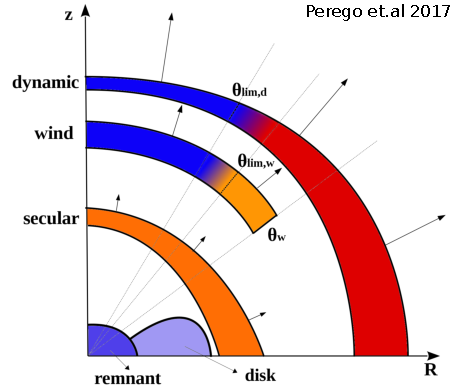
\includegraphics[height=5cm]{phd_figs/mkn__albino2.pdf}
            
            \hspace*{10mm} Ejecta compoenents in \texttt{MKN}
%            \caption{Graphic representation of the analyzed
%                ejecta profiles for isotropic and anisotropic cases
%                from an azimuthal perspective and for a fixed moment of time.
%                The black dot represents the remnant and the dashed line is the projected orbital
%                plane of the binary. The shadowed areas describe the ejecta profiles: the shape
%                characterizes the mass distribution, while the colors refer to 
%                the prior assumptions on the opacity parameter.
%                In particular, blue regions denote opacities lower than $5~\igscm$,
%                red regions refer to opacities greater than $5~\igscm$,
%                and oranges areas indicate a broadly distributed opacity.
%                All shells are isotropically expanding with a constant velocity.
%                (Adapted from \citet{Breschi:2021wzr})
    }};
}

%\texttt{MKN} code
%\uncover<1->{ % <-> |
%    \node (t2) [anchor=center,scale=1,opacity=1] at ([shift={(-3.8cm,-1.8cm)}]current page.center){
%        \parbox{0.6\textwidth}{
%            \begin{itemize}
%            \item multicomponent, anisotropic semi-analytical 
%            \end{itemize}
%    }};
%}

\end{tikzpicture}

\end{frame}



%% --------------------------------------------------------------
%%
%% Results
%%
%% --------------------------------------------------------------

%\begin{frame}{EM signature of the \swind{}} %% ---------- title 
%
%\begin{tikzpicture}[overlay,remember picture]
%
%\uncover<1->{ % <-> |
%    \node (t1) [anchor=center,scale=1,opacity=1] at ([shift={(-4.1cm,1.0cm)}]current page.center){
%        \parbox{0.55\textwidth}{
%            Dynamical ejecta cannot explain early blue emission \\
%            
%            Contribution from the \swind{} is natural
%            
%    }};
%}
%
%
%
%\uncover<1->{ % <-> |
%    \node (img1) [anchor=center,scale=1,opacity=1] at ([shift={(3.4cm,-0.2cm)}]current page.center){
%        \parbox{0.5\textwidth}{
%            \includegraphics[height=5.5cm]{kilonova/mkn_dd2_band.pdf}
%%            Bolometric kN light curves in three representative bands from blue to
%%            infrared for the two simulations with turbulence viscosity compared to
%%            \AT{} data from~\citep{Villar:2017wcc}.
%%            The color gradient is the effect related to different
%%            \ac{SWW} masses, that suggests possible variations of the light
%%            curves for different \ac{BNS}. The band is computed by extracting the
%%            \ac{SWW} mass from DD2 every $10$~ms until the end of the simulation, and
%%            then by linearly extrapolating the data to $250$~ms.
%%            (Adapted from \citet{Nedora:2019jhl})
%    }};
%}
%
%Low opacity, fast \ac{SWW} 
%\uncover<1->{ % <-> |
%    \node (t2) [anchor=center,scale=1,opacity=1] at ([shift={(-3.8cm,-1.8cm)}]current page.center){
%        \parbox{0.6\textwidth}{
%            \begin{itemize}
%            \item Dynamical ejecta cannot explain early blue emission
%            \item Probe of remnant dynamics, lifetime and EOS
%            \end{itemize}
%    }};
%}
%
%\end{tikzpicture}
%
%\end{frame}





\begin{frame}{Spiral-wave wind for the blue kilonova} %% ---------- title 

\begin{tikzpicture}[overlay,remember picture]

\uncover<1->{ % <-> |
    \node (t1) [anchor=center,scale=1,opacity=1] at ([shift={(-0.8cm,1.8cm)}]current page.center){
        \parbox{1.0\textwidth}{
            \begin{itemize}
            \item Dynamical ejecta cannot explain early blue emission
            \item Probe of remnant dynamics, lifetime and EOS
            \end{itemize}
    }};
}

\uncover<1->{ % <-> |
    \node (img1) [anchor=center,scale=1,opacity=1] at ([shift={(-2.0cm,-1.65cm)}]current page.center){
        \parbox{0.5\textwidth}{
            \includegraphics[height=5cm]{phd_figs/ejecta_dyn/summary/ej_mej_yeej_our2.pdf}
    }};
}

\uncover<1->{ % <-> |
    \node (img1) [anchor=center,scale=1,opacity=1] at ([shift={(3.8cm,-1.5cm)}]current page.center){
        \parbox{0.5\textwidth}{
            \includegraphics[height=5.15cm]{phd_figs/kilonova/mkn_dd2_band.pdf}
    }};
}


\end{tikzpicture}

\end{frame}

%\begin{figure*}[t]
%    \centering 
%    \includegraphics[width=0.48\textwidth]{ejecta_dyn/summary/ej_mej_vej_our2.pdf}
%    \includegraphics[width=0.48\textwidth]{ejecta_dyn/summary/ej_mej_yeej_our2.pdf}
%    \caption{
%        Summary of the ejecta properties of our models.
%        %
%        Diamonds mark the dynamical ejecta, crosses include the
%        contribution of the \swind{} for the long-lived models, 
%        triangles are an estimate of the total ejecta mass on a secular
%        timescale, assuming $40\%$ of the disk mass is unbounded on
%        secular timescales.         
%        The ejecta mass is shown is terms of the mass-averaged velocity
%        (left) and of the averaged electron fraction (right).
%        %
%        The filled blue and red patches are the expected values of
%        ejecta mass and velocity for blue and red components of
%        AT2017gfo compiled by \cite{Siegel:2019mlp}, based on
%        \cite{Villar:2017wcc}. 
%        Adopted from \citet{Nedora:2020pak}.
%    }
%    %
%    \label{fig:ejecta:dyn:ds_sww}
%\end{figure*}
